\chapter{Analysing the tree in Python}
\label{ch:python}

\begin{willdo}
\begin{itemize}
  \item Open a \musrSim\ ROOT file in Python with \code{uproot} --- no ROOT installation required.
  \item Handle the per-hit jagged arrays correctly with \code{awkward}.
  \item Plot an energy spectrum and fit the muon lifetime.
  \item Package the boilerplate into a small, reusable loader.
\end{itemize}
\end{willdo}

You can analyse \musrSim\ output entirely in Python. The \code{uproot} library reads ROOT files without a ROOT installation, and \code{awkward} gives you fast, NumPy-like operations on the variable-length hit arrays. This chapter builds a complete analysis of the \code{first_sim.mac} output in small pieces. The finished scripts live in \code{doc/scripts/}.

\section{Opening the file}
Install the toolkit once (Section~\ref{sec:conda}), then open the tree by name.

\begin{lstlisting}[style=py,caption={Reading tree \texttt{t1} into arrays}]
import uproot
import awkward as ak
import numpy as np

t = uproot.open("data/musrSim_jp000.root")["t1"]    # the tree is always called t1
print(t.num_entries, "events,", len(t.keys()), "branches")

# Per-hit branches come back as jagged awkward arrays,
# event-level branches as flat arrays.
data = t.arrays(["det_n", "det_ID", "det_edep", "det_time_start",
                 "muDecayTime", "muDecayDetID"], library="ak")
\end{lstlisting}

For the reference run this prints \code{19991 events, 80 branches}.

\begin{keypoint}
\code{det_edep} is \emph{jagged}: event 0 might have two hits and event 1 one. You cannot treat it as a flat column until you either flatten it or select one hit per event. Reaching for \code{np.array(det_edep)} on a jagged branch is the first mistake most people make --- use \code{awkward} instead.
\end{keypoint}

\section{Energy spectra: flattening and masking}
To histogram the energy of every hit, flatten the jagged array. To histogram one counter, mask on \code{det_ID} \emph{before} flattening, so the mask and the data stay aligned.

\begin{lstlisting}[style=py,caption={All-hit spectrum, and a single-counter spectrum}]
import matplotlib.pyplot as plt

all_edep  = ak.flatten(data.det_edep)              # 1-D array of all hits
mask      = data.det_ID == 1                        # jagged boolean, same shape as det_edep
edep_slab = ak.flatten(data.det_edep[mask])         # mask, THEN flatten

fig, ax = plt.subplots(figsize=(6, 4))
ax.hist(np.asarray(all_edep),  bins=100, range=(0, 15), histtype="step", label="all hits")
ax.hist(np.asarray(edep_slab), bins=100, range=(0, 15), histtype="step", label="det_ID == 1")
ax.set_xlabel("Energy deposit [MeV]"); ax.set_ylabel("Hits / bin"); ax.legend()
fig.savefig("edep_spectrum.png", dpi=150)
\end{lstlisting}

\begin{pitfall}
Order matters: \code{ak.flatten(det_edep)[mask]} is wrong, because once \code{det_edep} is flattened the per-event mask no longer lines up with it. Always apply the jagged mask first (\code{det_edep[mask]}) and flatten the result.
\end{pitfall}

To separate the prompt muon hits from the delayed positron hits of Figure~\ref{fig:edep}, mask on time in exactly the same way: \code{data.det_edep[data.det_time_start < 0.01]} keeps hits that started within \SI{10}{ns}.

\section{The muon lifetime}
\code{muDecayTime} is an event-level scalar (in \si{\micro s}), so no flattening is needed --- but you must cut the sentinel for muons without a recorded decay, and you will usually select muons that stopped in a particular volume.

\begin{lstlisting}[style=py,caption={Histogram and fit the muon decay time}]
from scipy.optimize import curve_fit

t_us = np.asarray(data.muDecayTime)
good = np.asarray((data.muDecayDetID == 1) & (data.muDecayTime > 0))   # stopped in the slab
t_us = t_us[good]

counts, edges = np.histogram(t_us, bins=100, range=(0, 15))
centres = 0.5 * (edges[:-1] + edges[1:])

def decay(t, N0, tau, bkg):
    return N0 * np.exp(-t / tau) + bkg

popt, pcov = curve_fit(decay, centres, counts, p0=[counts.max(), 2.2, 1.0],
                       sigma=np.sqrt(counts + 1), absolute_sigma=True)
tau, dtau = popt[1], np.sqrt(pcov[1, 1])
print(f"tau = {tau:.4f} +/- {dtau:.4f} us   (PDG: 2.1970 us)")
\end{lstlisting}

On the 19\,990 muons of the reference run this gives \(\tau = \SI{2.214(20)}{\micro s}\), within one standard deviation of the PDG value (Figure~\ref{fig:lifetime}).

\begin{figure}[h]
\centering
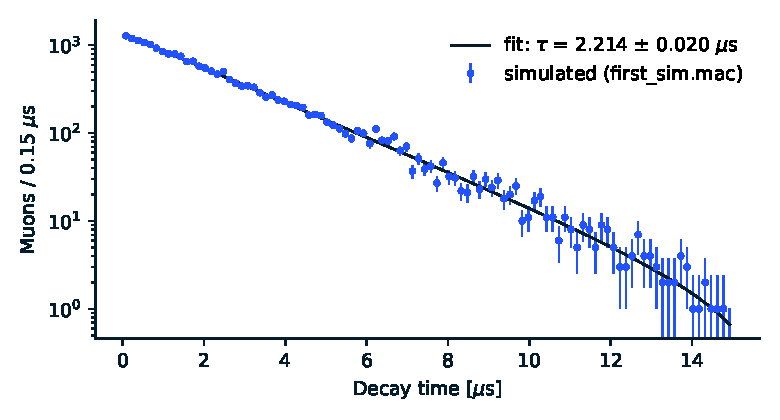
\includegraphics[width=0.78\textwidth]{figures/lifetime.pdf}
\caption{Decay-time distribution of the muons stopped in the slab in \texttt{first\_sim.mac}, with the exponential-plus-constant fit.}
\label{fig:lifetime}
\end{figure}

\begin{physics}
A pure positive-muon sample recovers the free mean life, \(\tau_{\mu^+}\approx\SI{2.197}{\micro s}\). Fit a negative-muon run (\code{/gun/primaryparticle mu-}, with \code{G4MuonMinusCapture} in the physics block) and you will measure something shorter: a \(\mu^-\) stopped in matter can be captured by a nucleus, so its disappearance rate is the sum of decay and capture, and the shift depends strongly on \(Z\) of the stopping material. Seeing that shift emerge from your own simulation is a satisfying check that the physics list is doing its job.
\end{physics}

The complete version of this analysis, which also produces both plots, is \code{doc/scripts/first_analysis.py}; run it from \code{build/run} as \code{python ../../doc/scripts/first_analysis.py}.

\section{A reusable loader}
Wrap the boilerplate once so every later analysis starts from a clean function.

\lstinputlisting[style=py,caption={\texttt{doc/scripts/load.py} --- a small, reusable entry point}]{scripts/load.py}

\begin{tip}
For a whole run directory, \code{uproot.concatenate("data/musrSim_jp201_job*.root:t1", branches, library="ak")} reads and stitches many files at once --- the natural next step when you split a big job across a batch farm (Section~\ref{sec:scale}).
\end{tip}

\begin{recap}
\begin{itemize}
  \item \code{uproot} opens \code{t1} with no ROOT install; per-hit branches are jagged \code{awkward} arrays.
  \item Mask on \code{det_ID} (or time) before flattening; flatten only when you want a 1-D histogram.
  \item \code{muDecayTime} fits to \(\approx\SI{2.197}{\micro s}\) for \(\mu^+\); cut the sentinels first.
  \item A tiny \code{load()} / \code{counter()} pair removes the boilerplate from every future script.
\end{itemize}
\end{recap}
\nextchap{fields, the physics list, and running at scale}
